\documentclass[UTF8,a4paper,11pt,fontset=fandol]{ctexart}

\usepackage[a4paper,margin=2.3cm]{geometry}
\usepackage{hyperref}
\usepackage{amsmath}
\usepackage{booktabs}
\usepackage{tikz}
\usepackage{graphicx}

\title{“智变：AI 与新质生产力”展示网站}
\author{可视化导论第二次作业}
\date{2026年10月8日}

\hypersetup{colorlinks=true,linkcolor=blue,urlcolor=blue}
\definecolor{storyblue}{HTML}{5065BB}
\definecolor{storymint}{HTML}{287A68}
\definecolor{storypaper}{HTML}{F0F3FA}
\definecolor{storygreen}{HTML}{EDF5F2}

\begin{document}

\maketitle

\section{作品概述}

本次作业以“人工智能怎样成为新质生产力”为题，做了一个中英双语交互展示网站。主页面用一条连贯的滚动叙事，从工作流程讲到产业应用、研究证据、技术扩散和实现条件，最后把问题交给读者：生产环节加速之后，整条流程真的省下了时间？“数据与方法”页面把来源、统计说明、研究限制都列了出来，还提供数据下载。主线共六章、21 个步骤，其中有五个产业案例。

站点入口：\url{https://vis.starlab.top/hw02/}。

\section{关键亮点}

\subsection{六个章节串成一条问题链}

六个章节按读者会追问的顺序排下来：第一章拆开检索、生产、复核、交付的工作流；第二章走进制造、医疗、农业、科研、服务五个现场；第三章用研究检验效率和质量到底变了没有；第四章分清采用率、组织差异和投资背景各自在说什么；第五章补上数据、算力、能源和人的责任；第六章交给读者自己调参数验证。

顺序这样排，读者的理解就会从“AI 能做什么”走到“什么条件下才有收益”。开头看到 AI 能帮着出答案，往后会遇到具体任务的研究数据，到实验里才发现：生产变快不等于总工时变少，多出来的复核可能把收益吃掉。

主线每一步只提一个观察重点，图表始终跟着当前文字，按钮都集中到章末，第一次阅读就能一路顺畅读到底。想往深处走的读者，章末“展开完整图表与操作”里还有一批更细的图：产业部分的案例可以切换，网络和矩阵也能对照着看，另有机器人、医疗、气象和科学发现几张图；研究部分把客服效率、写作耗时、质量评分和开发者研究分别比较；扩散与边界部分展示采用率、企业规模、投入、能源和可能被 AI 触及的工作。14 类图表都在这里，实验区默认展开。

每张图表都带着标题、单位和来源，读者一眼就能看出它在回答什么问题；不同调查对象、不同单位的数字各成一张图，各答各的问题。

\subsection{封面与章节海报}

封面铺了一张粒子网络：光点缓慢漂移，鼠标靠近时点亮周围几颗，滚动离开封面时整张网收拢成一条亮线。结尾复用同一张网，进入视口后排成网格，然后停下。粒子从当前主题里取色，切换明暗时立即重绘。

每章开头是一屏海报。右侧一枚描边巨号章节数字，随滚动从描边填充成实色；标题背后一块斜切条纹色块，从左侧擦出；章节标题逐字上浮，章节位置、章节说明和 STEPS／SOURCES／MODE 元数据依次跟进，底部一条跑马条循环滚过本章的步骤标题。继续往下滚，海报向上收拢，把画面让给舞台。

标题动效分两种：章节标题逐字上浮，封面和结尾的标题只做轻微显现——淡入的同时上移几个像素。文字一开始就是可读的原文，入场只加位移和透明度，没有加载等待。

\subsection{每章一个固定的舞台}

桌面端每章都有一块固定的图区：文字和图形停在原地，滚动只管往前推进画面，每张图画完都能停在视野里读完。往回滚就能回到上一段，滚轮照常工作，翻到哪儿全由读者说了算。换段时上一段淡出，新一段顺着滚动方向擦入、由虚变实，标题、正文和来源依次进场；连续滚动时平滑接续，快速跨段时直接定位，读者也能随时倒回。

六章根据内容关系选择三种桌面版式（图~\ref{fig:layouts}）：工作流程和实现条件左右分栏，产业与扩散章把文字和图表的左右位置对调，证据与实验章则是上方说明、下方通栏图表。说明区按实际文案长度自然撑开，图表使用余下空间，装在带 HUD 四角括号的独立面板里，边框取本章的强调色。

配色按全站的明暗主题各做一套：深色以深蓝为底，强调色用电光青、黄绿、紫和品红；浅色换成冷白底、墨蓝文字，同一组强调色压深后继续用。主线、章末探索、资料页和图表都跟着主题切换，粒子网络也会即时换色。

动画跟着内容关系变化：AI 支线接入检索和生产节点，圆点沿连接移动；采用率沿年份展开；研究结果点从各自基准移到结果位置；能源柱从共同基线升起，历史估计与虚线预测依次出现；实验条带随着生产与复核时间连续变化。坐标轴、基准与背景轨道保持完整，读者能在变化中保留参照。

每章末尾都多留出一个舞台高度的滚动距离，让最后一张图停在画面上，读者可以从容看完；图完整停留过之后，舞台再退场。通栏版式把说明带和图表装进同一个固定框里，两者同进同退，标题始终贴着图表。产业网络始终保留完整连线，只用颜色强调当前案例，五个现场的共同能力和责任差异一对比就看得出来。

\begin{figure}[htbp]
  \centering
  \begin{tikzpicture}[font=\small,
    copy/.style={draw=storyblue!55,fill=storypaper,rounded corners=2pt},
    plot/.style={draw=storymint!60,fill=storygreen,rounded corners=2pt}]
    \draw[gray!45,rounded corners=3pt] (0,0) rectangle (4.4,2.6);
    \draw[copy] (.2,.25) rectangle (1.7,2.35);
    \node[align=center] at (.95,1.3) {固定\\正文};
    \draw[plot] (1.95,.25) rectangle (4.2,2.35);
    \node[align=center] at (3.075,1.3) {流程\\图表};
    \node at (2.2,-.35) {工作流程／实现条件};

    \draw[gray!45,rounded corners=3pt] (5.2,0) rectangle (9.6,2.6);
    \draw[plot] (5.4,.25) rectangle (7.65,2.35);
    \node[align=center] at (6.525,1.3) {关系\\图表};
    \draw[copy] (7.9,.25) rectangle (9.4,2.35);
    \node[align=center] at (8.65,1.3) {固定\\正文};
    \node at (7.4,-.35) {产业应用／技术扩散};

    \draw[gray!45,rounded corners=3pt] (10.4,0) rectangle (14.8,2.6);
    \draw[copy] (10.6,1.6) rectangle (14.6,2.35);
    \node at (12.6,1.975) {固定说明带};
    \draw[plot] (10.6,.25) rectangle (14.6,1.35);
    \node at (12.6,.8) {通栏图表};
    \node at (12.6,-.35) {研究证据／流程实验};
  \end{tikzpicture}
  \caption{三种桌面版式的结构示意。通栏说明带和图表共用一个固定边界。}
  \label{fig:layouts}
\end{figure}

\subsection{随手可调的流程实验}

实验台有四个参数：任务数量、AI 参与比例、参与任务的加速倍率，以及每项任务的额外复核时间。需求、生产、复核、交付四段按同一时间比例排开，拖动滑杆就能同时看到每段长度、总工时和净节省的变化。点一下播放，四段流程会自己走一遍；敏感性图显示参与比例和收益的关系；复制出来的链接会带上这组参数，方便重复演示和分享。

模型把假设写明了：每项任务的需求整理、生产、原有复核、交付分别是 10、30、10、5 分钟；AI 只加速生产环节，额外复核则要算进每一项任务。设任务数为 $n$，AI 参与比例为 $a\in[0,1]$，加速倍率为 $s$，额外复核为 $r$ 分钟，则
\begin{align*}
  T_0 &= 55n,\\
  T_{\mathrm{AI}} &= n\left[10+30\left(1-a+\frac{a}{s}\right)+10+r+5\right],\\
  \eta &= \frac{T_0-T_{\mathrm{AI}}}{T_0}\times100\%.
\end{align*}
两种总工时都按分钟算，这几个时间值都是为教学设定的。模型算的是工时：并行处理和质量变化都还没有算进去；从省下的工时到实际的经济收益，中间还隔着不少环节。

默认设置是 20 项任务、60\% 参与、3 倍加速、额外复核 4 分钟，原流程 1100 分钟，AI 协作 940 分钟，净节省约 14.5\%。表~\ref{tab:presets} 列出三组预设：复核便宜时节省明显，复核昂贵时会变成负收益，参与比例过低则可能抵不过复核成本。滚动位置和用户参数分开管理，回看前文时，已经调好的实验保持原样。

\begin{table}[htbp]
  \centering
  \small
  \begin{tabular}{lrrrr}
    \toprule
    教学预设 & AI 参与比例 & 加速倍率 & 额外复核 & 净省工时 \\
    \midrule
    低复核成本 & 80\% & $3\times$ & 1 分钟 & 27.3\% \\
    高复核成本 & 80\% & $3\times$ & 20 分钟 & $-7.3\%$ \\
    低参与比例 & 15\% & $3\times$ & 4 分钟 & $-1.8\%$ \\
    \bottomrule
  \end{tabular}
  \caption{三组预设用同一个模型，任务数都是 20。负数表示 AI 协作流程耗时更多。}
  \label{tab:presets}
\end{table}

\subsection{结论都能追到来源和统计说明}

“数据与方法”页面（\url{https://vis.starlab.top/hw02/sources/}）收了 30 条指标记录、五个产业案例和 21 个来源。读者按关键词搜来源，也能按统计、研究、案例与概念筛选；展开每条指标，还能看到样本、期间和限制。主线的脚注给出两个入口——原始来源和本站统计说明，点进去直接落到对应的来源或指标，省去了从图表一路找回去的麻烦。

图表和下载用的 CSV 出自同一份 JSON，图里的数字和下载文件始终一致。标注上分得很细：实测数据和研究结论分开，历史估计和未来预测分开，机制示意和教学模拟分开。数据中心用电的历史估计与未来情景分别标明，可能被 AI 触及的工作不等于失业概率，产业网络的连线只表示能力上的联系，与效果强弱无关。来源也就成了可视化说明的一部分，读者在图上就能看到结论的出处。

\subsection{双语、窄窗口与降级}

中文和英文的章节、数据、操作一一对应，共用全站的导航和语言切换，深色与浅色两套主题各配一份。章节条给出目录、当前位置和阅读进度，锚点直接跳到某一步；切换语言时保留阅读位置和实验参数，底色、文字、图表和控件都跟着主题走。

窄窗口另做了一套版式：宽度和高度都够，就改成上方紧凑固定图、下方正文；高度不够，或者系统开了“减少动态效果”，就回到按步骤排列的图文。禁用 JavaScript 时，正文、数据表、产业案例、默认实验结果和来源仍然可读，章节链接和原生详情展开也还能用。

网站用 Astro 做成静态页面，D3 画图，GSAP 管滚动，粒子网络用 Canvas 画在封面和结尾。正文和数据先直接渲染出来，图形等快滚到眼前再加载；图形按最终尺寸提前占好高度，减少加载带来的位置跳动。

\section{设计思路总结}

这套网站想帮读者形成自己的判断。滚动叙事按顺序摆出问题，交互图表摆出证据，流程实验让人亲手验一遍假设，来源和统计说明交代结论能用到哪里。文字和图形什么时候停留、什么时候切换、什么时候退出，都跟着阅读节奏走，读者既能顺着主线看懂全貌，也能停下来自己探索。

效率要靠整条流程一起改善，质量得反复验证，创新离不开试错。可视化能做的，是把这些条件和关系摆到读者眼前——看得见，比得了，也能自己动手改。

\section{页面截图}

四张截图取自 1440×900 的桌面视口，滚动与动效见演示视频。

\begin{figure}[!htbp]
  \centering
  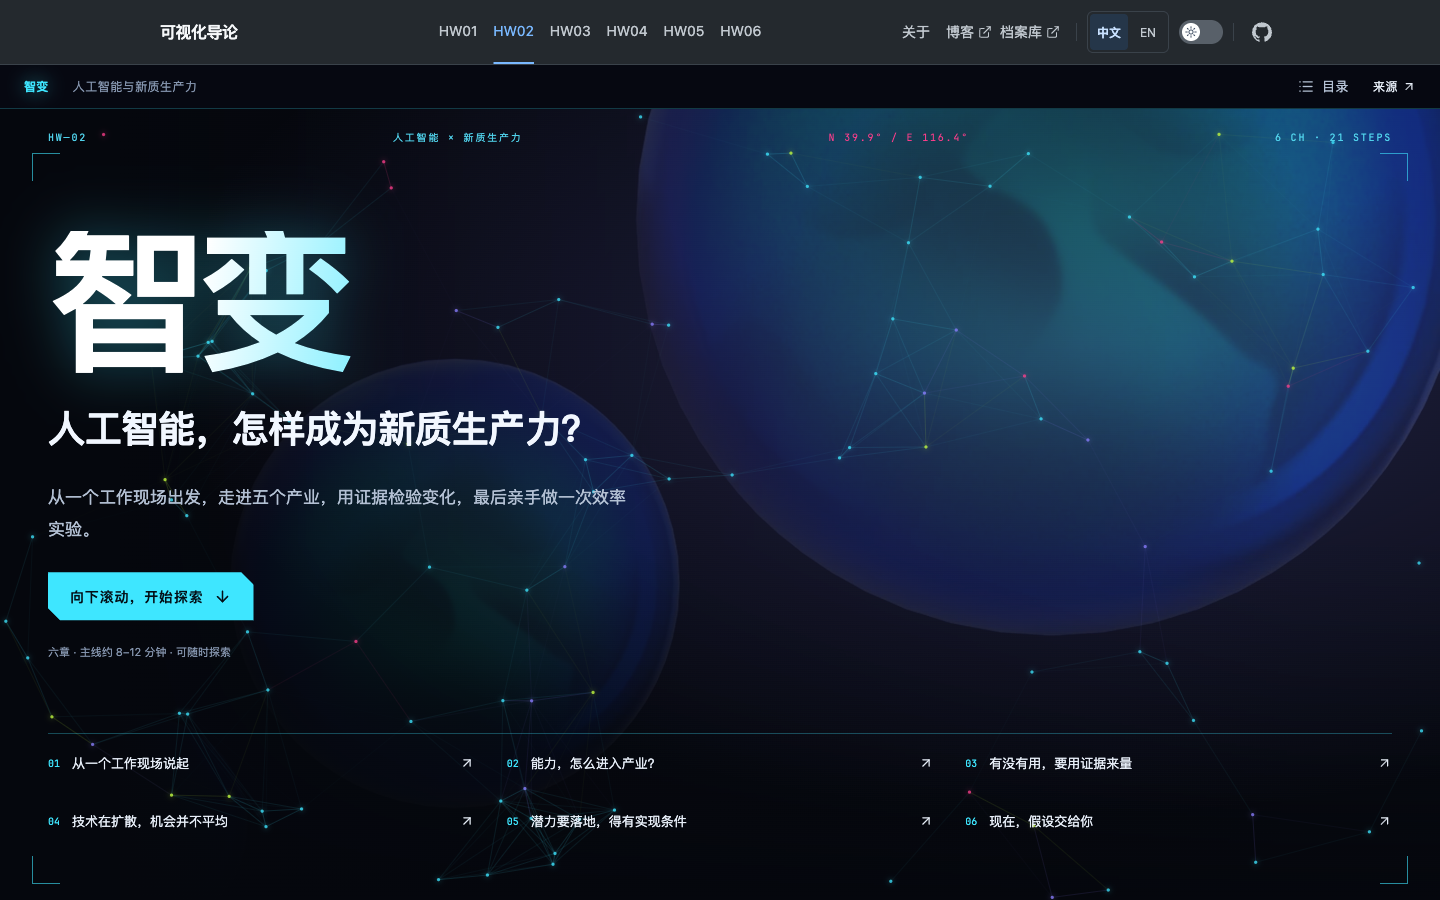
\includegraphics[width=0.487\textwidth]{images/cover-dark.png}\hfill
  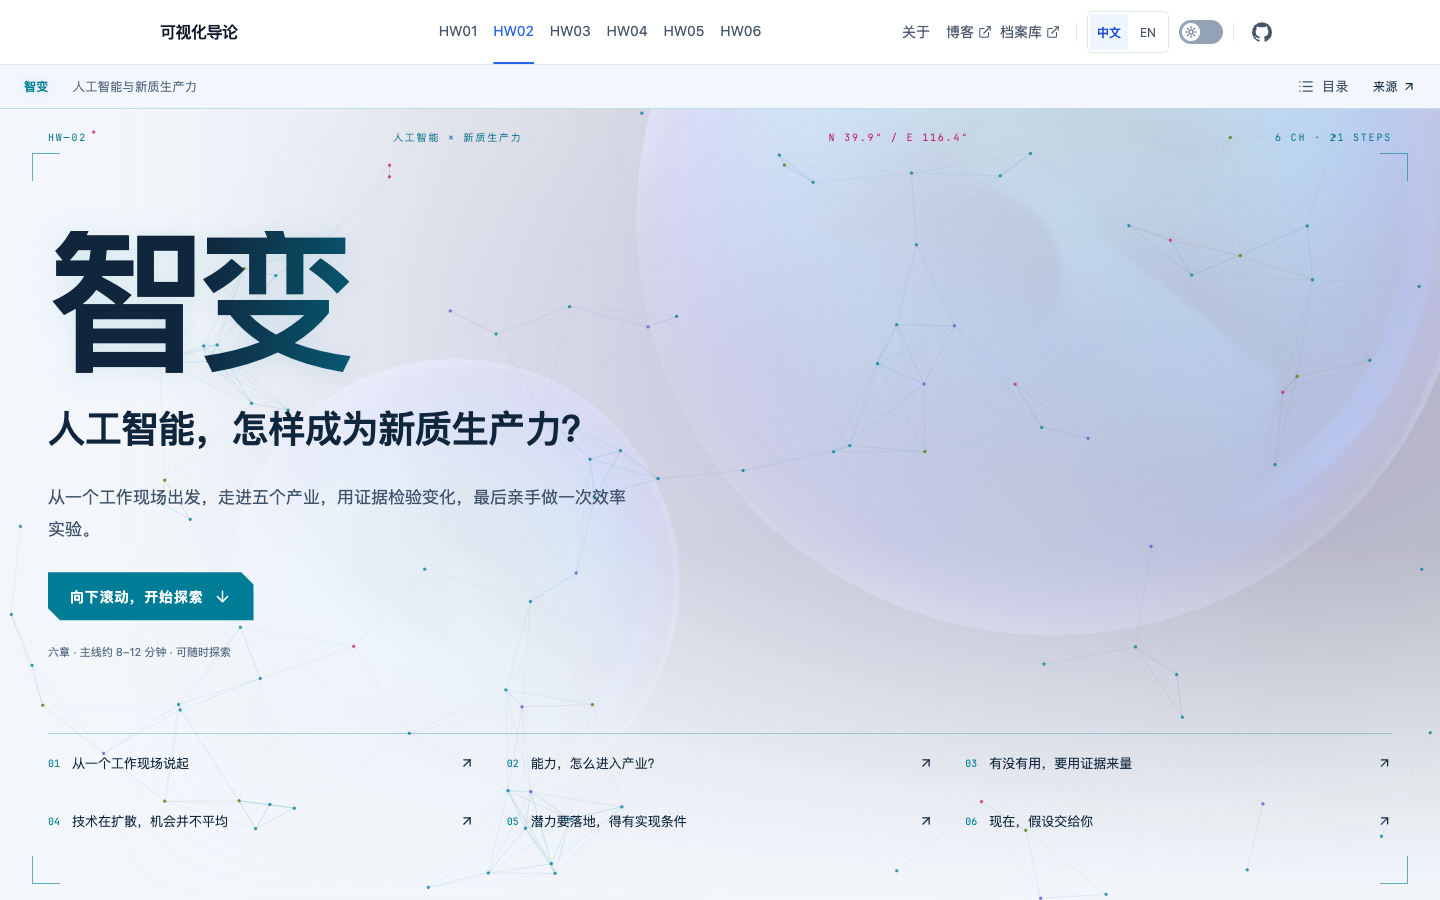
\includegraphics[width=0.487\textwidth]{images/cover-light.png}
  \caption{封面。左为深色主题，右为浅色主题；粒子网络、四角括号和顶部 HUD 跟着主题换色。}
  \label{fig:cover}
\end{figure}

\begin{figure}[!htbp]
  \centering
  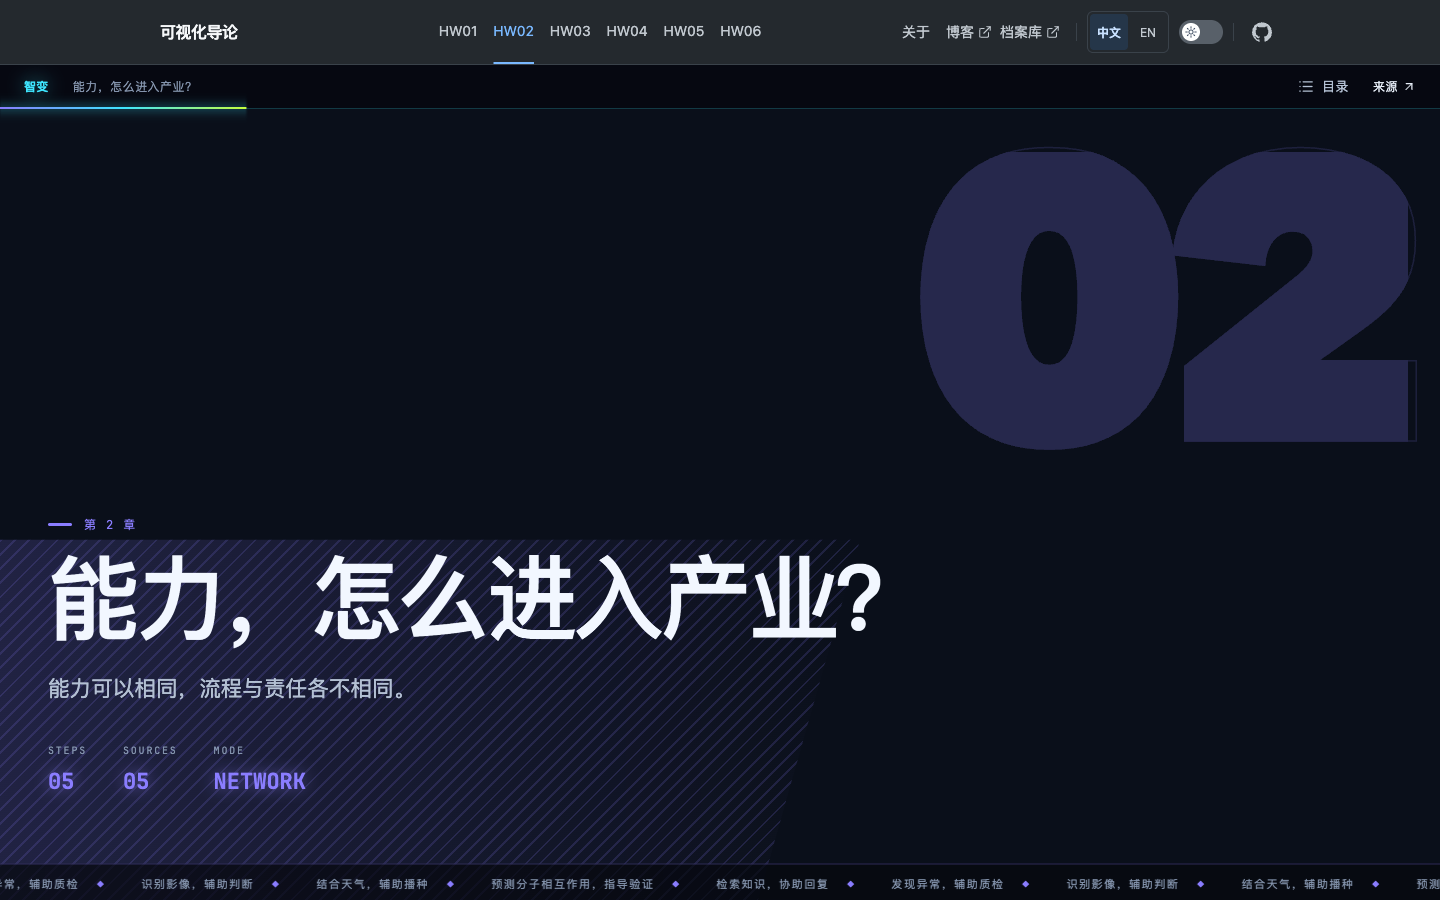
\includegraphics[width=0.487\textwidth]{images/chapter-poster.png}\hfill
  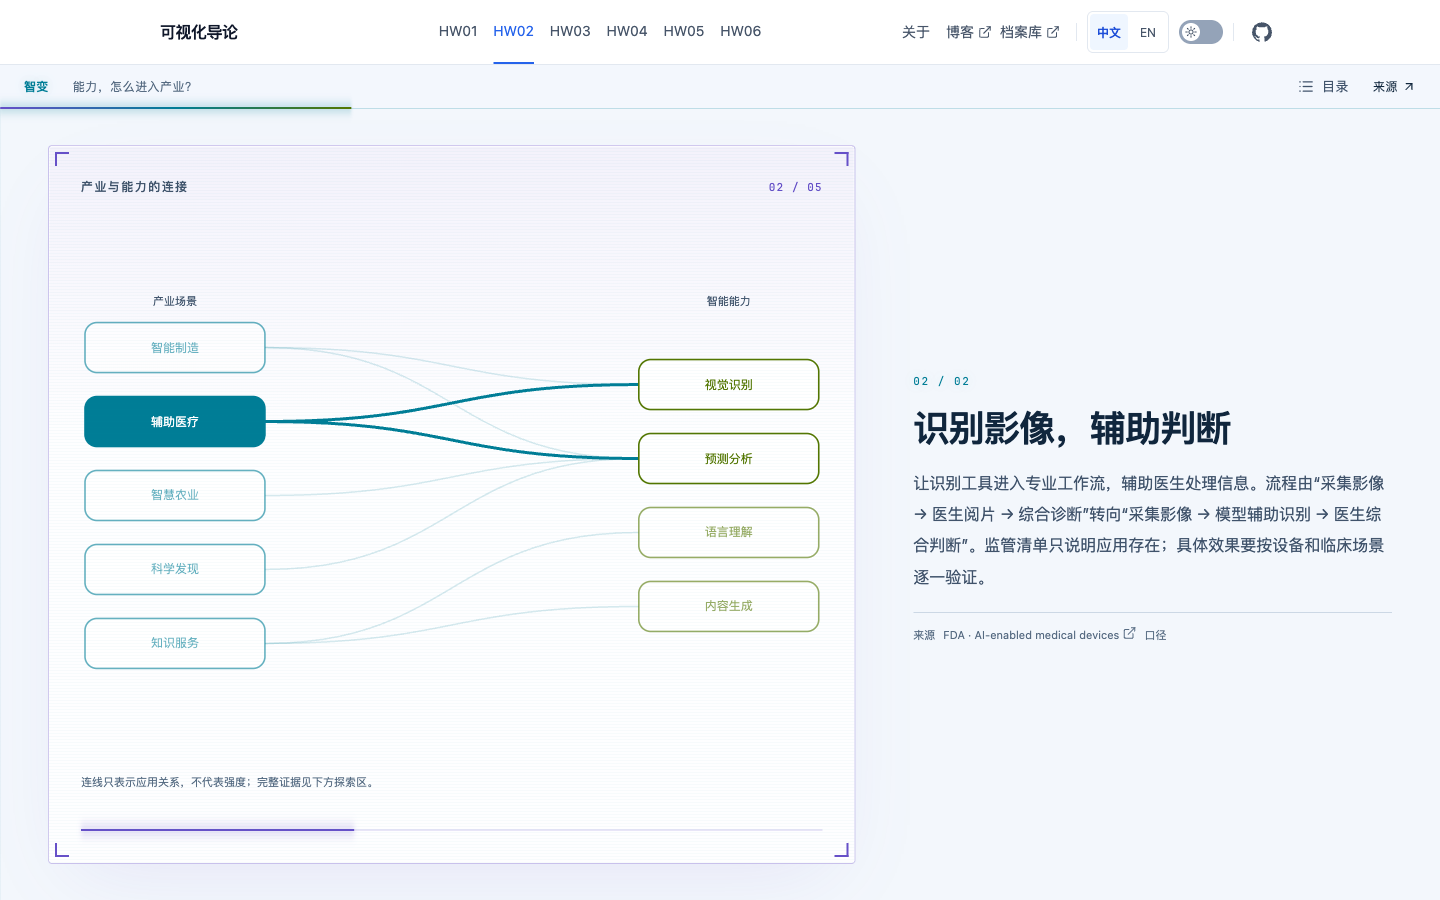
\includegraphics[width=0.487\textwidth]{images/industry-stage.png}
  \caption{左：深色主题下的第二章海报，描边巨号数字、斜切条纹色块与元数据。右：浅色主题下的医疗案例舞台，图表装在带 HUD 四角括号的独立面板里。}
  \label{fig:poster-stage}
\end{figure}

\end{document}
